\documentclass[14pt,aspectratio=1610]{beamer}
\usepackage[utf8]{inputenc}
\usepackage[ngerman]{babel}
\uselanguage{ngerman}
\languagepath{ngerman}
\usetheme{simple}
\usecolortheme{whiteonblack}
\usepackage{array}
\usepackage{aurl}
\daurl{meta}{http://www.snik.eu/ontology/meta/}
\daurl{ob}{http://www.snik.eu/ontology/ob/}
\daurl{bb}{http://www.snik.eu/ontology/bb/}
\usepackage{url}
\usepackage{graphicx}
\usepackage{csquotes}
\usepackage{amssymb}
\usepackage{pifont}
\newcommand{\xmark}{\ding{55}}%
\newcolumntype{H}{>{\setbox0=\hbox\bgroup}c<{\egroup}@{}} % comment out columns
\date{25. März 2022}
\author{\texorpdfstring{Konrad Höffner\newline\url{konrad.hoeffner@imise.uni-leipzig.de}}{Konrad Höffner}}
\title{Vorstellung und Stand der Technik}
\subtitle{}
\begin{document}

\begin{frame}
\titlepage
\end{frame}

\begin{frame}{A Review of the Semantic Web Field (2021)}
\begin{itemize}
\item frühe 2000er: Ontologien
\item $\approx$ 2006--2012: \textbf{Linked (Open) Data}
\item 2021--heute: knowledge graphs, Industrie
\end{itemize}
\end{frame}

\begin{frame}{Linked Open Data}
\begin{itemize}
\item Fokus auf Nutzen für Anwender
\item simple Ontologien als Schema
\item offene Lizenzen, Wiederverwendung fördern
\item möglichst viele Werkzeuge und Schnittstellen
\item Technik und Entwicklung muss extrem effizient sein, da Personal und Mittel meist sehr stark auf Domänenexperten fokussiert sind
\item Technik meist teurer als auf dem freien Markt durch Verträge
\item Domänenexperten bringen Grundkenntnisse der Technologien mit aber keine Zeit, Interesse und Vertiefung auf Softwarentwicklung und Technikdetails
\end{itemize}
\end{frame}

\begin{frame}{Werkzeuge HITO: Health IT Ontology}
\end{frame}

\begin{frame}{}
\centering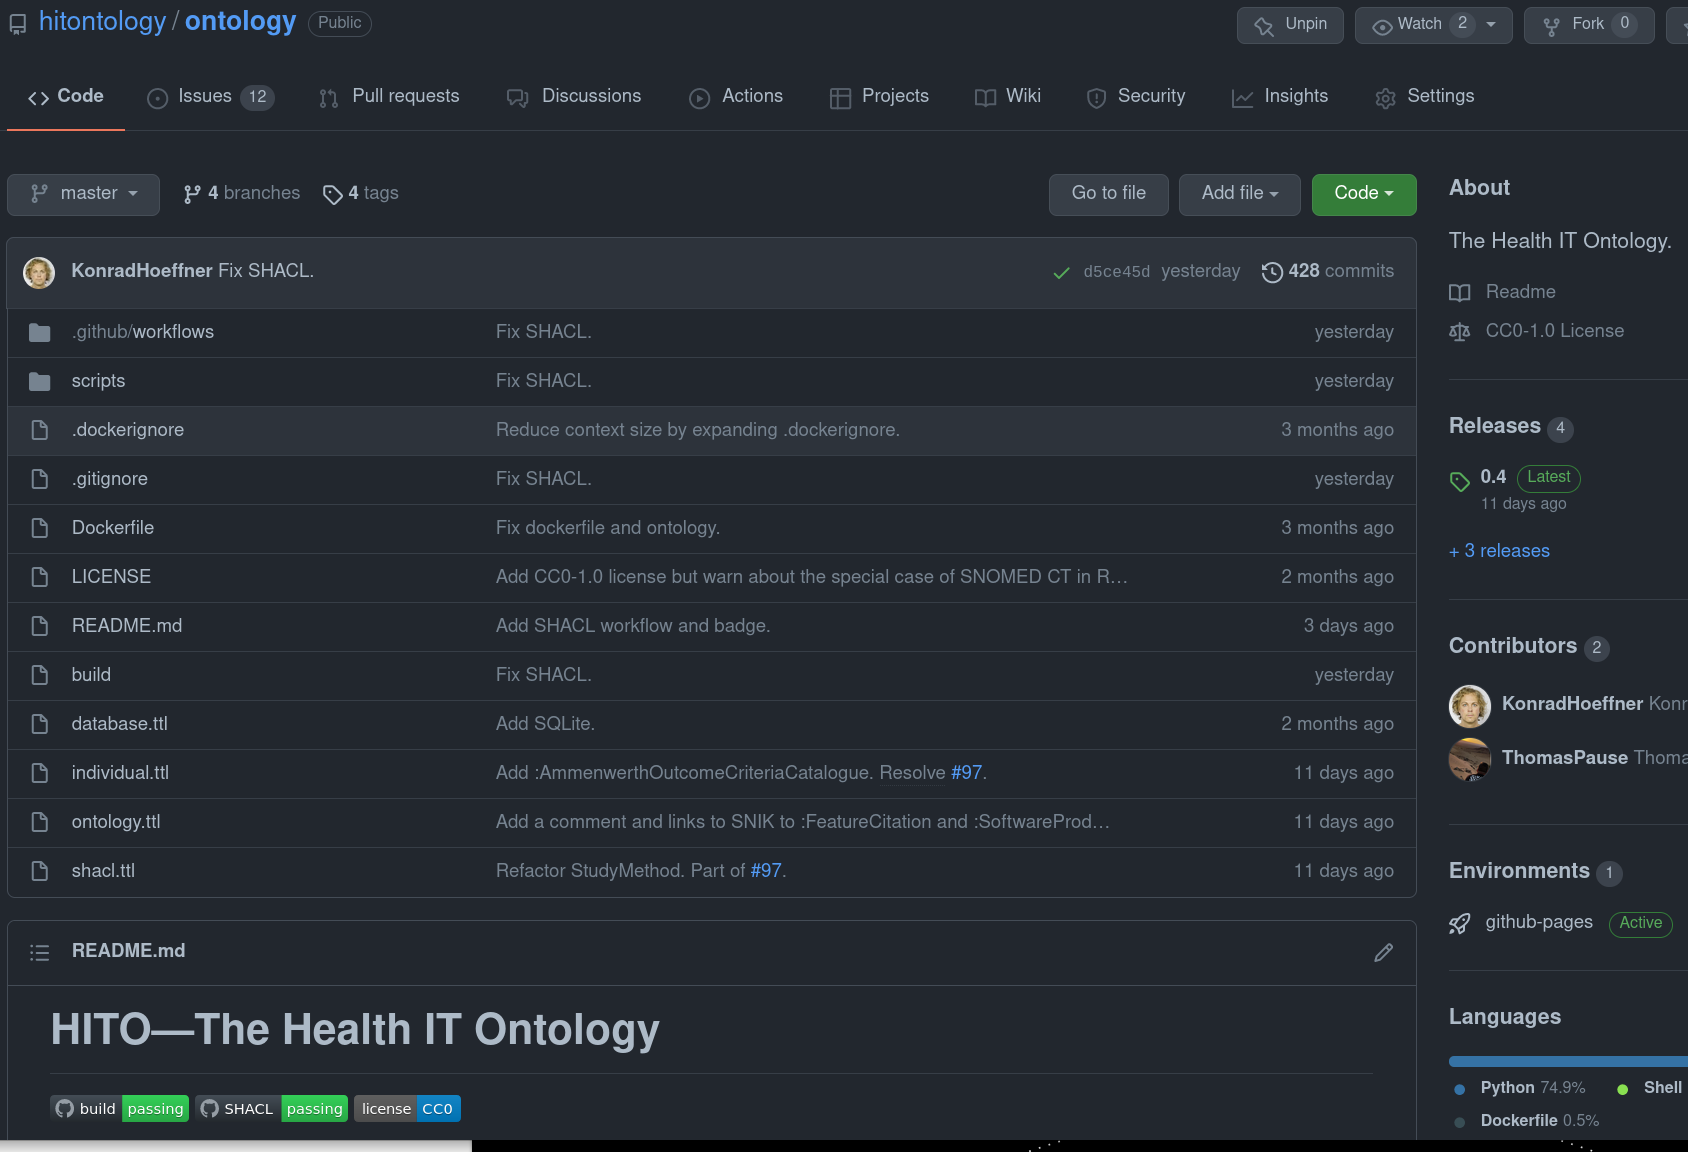
\includegraphics[width=1.05\textwidth,height=1.05\textheight,keepaspectratio]{img/github.png}
\end{frame}

\begin{frame}{}
\centering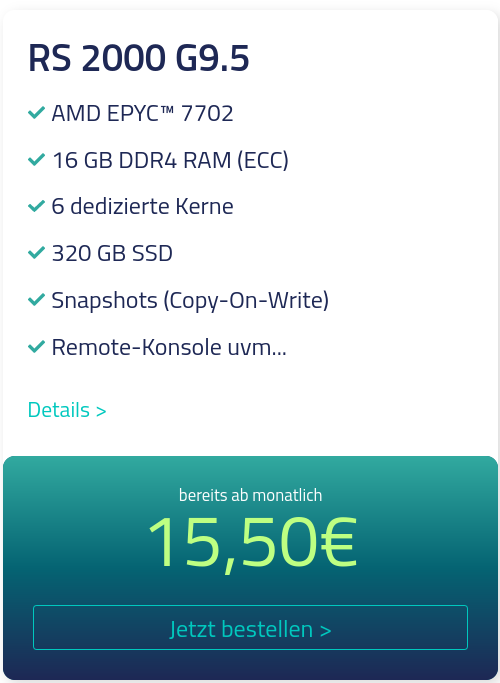
\includegraphics[width=1.05\textwidth,height=1.05\textheight,keepaspectratio]{img/netcup.png}
\end{frame}

\begin{frame}{}
\centering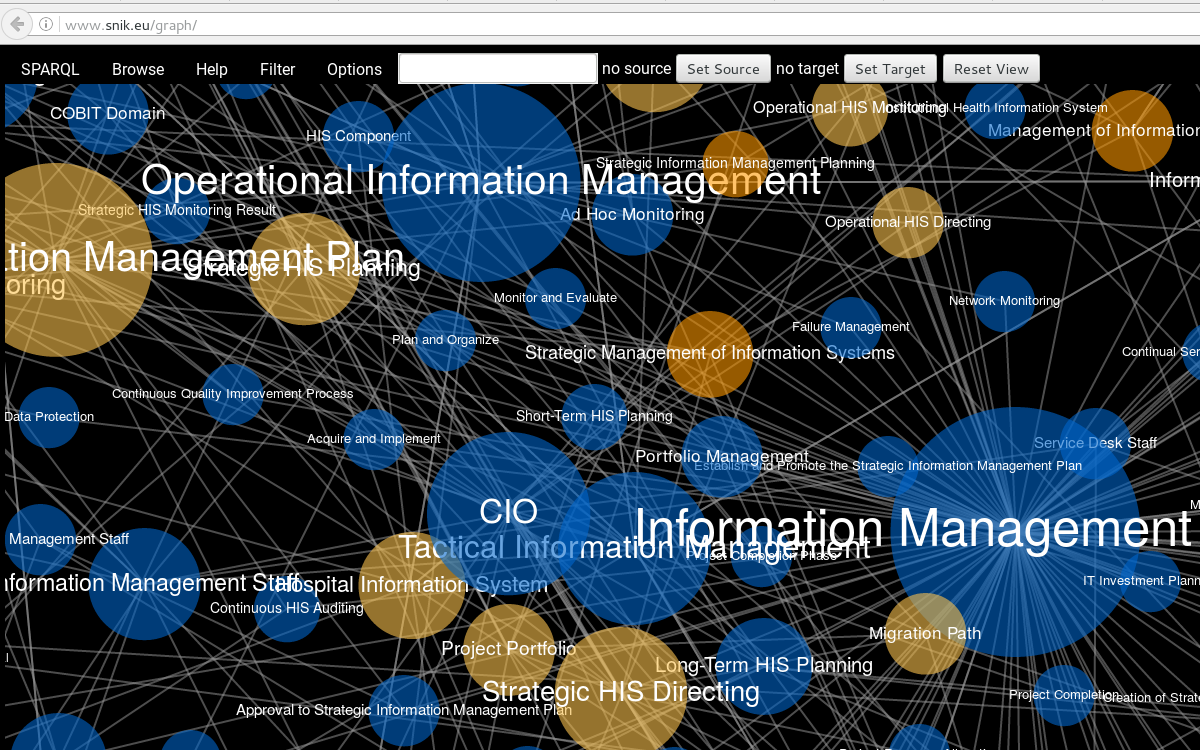
\includegraphics[width=1.05\textwidth,height=1.05\textheight,keepaspectratio]{../../2016/snik-projekttreffen/img/browser.png}
\end{frame}

\end{document}
